\chapter{Data collection}
This chapter discusses the following: the ethical considerations for this research \ref{Sec: Ethics}, followed by the survey design \ref{Sec:Privacy Notice} along with the relevant decision choices, and finally its implementation of the survey \ref{Sec: Implementation} including the pilot study \ref{Subsec: pilot study}, its analysis \ref{subsec: pilot analysis} and the final data collection procedure \ref{Subsec: Data collection}. The overview of this process can be seen in the Figure \ref{fig:methodology} 

\begin{figure}[tbp]
  \centering
  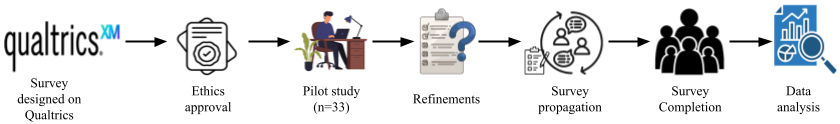
\includegraphics[width=1.0\textwidth]{methodology.png}
  \caption{Overview of the methodology.}
  \label{fig:methodology}
\end{figure}

\section{Ethical Considerations} \label{Sec: Ethics}

The study along with its overview, the consent notice being shown to the participants, data collection, storing, usage and deletion pipeline was sent to the University's Ethics Review Board (ERB) for approval, which was received with a suggestion to mention the demographic data being collected from the participants in the consent notice. Upon making this change, this study was fully compliant and following the standard ethical practices set by the GDPR. The participants are shown the consent notice, which consists of the information pipeline and point of contact among other things, as mentioned in Section~\ref{Sec:Privacy Notice}. The anonymous survey was conducted on a university-instance of the Qualtrics platform, ensuring that no personally identifiable information was collected from the participants including their geolocation/IP addresses. Any PII provided by the participants as part of the open-text responses in the survey would also be de-identified and removed prior to the analysis. Survey data is collected and stored on the internal servers in compliance with the data privacy practices for a period of 1 year post the completion of the work. The same information is also communicated clearly to the participants in the consent notice. 

\section{Survey Design} \label{Sec:Privacy Notice}

The survey consists of 29 questions and takes approximately 10 minutes for completion. The participants are initially shown the description of the project, contact information of the researchers and the consent notice. Consent notice contains the list of the demographic information being collected and provides information about their personally identifiable information (PII) not being collected in any form. It also mentions that any information voluntarily provided by the participants as part of their open-text responses would be removed. However, due to such anonymization, the participants are also informed that they cannot request for deletion of their data at a later stage. Additionally, they are explicitly informed that the participation is completely voluntary and that they could opt-out at any given point in time before clicking the `submit' button in the end. They were then asked to confirm that \begin{itemize}
    \item They were above the age of 18
    \item They were a citizen and/or a resident of India and use the Internet
\end{itemize}
Finally, the participants were asked to only proceed ahead if they had read the entire consent notice, agree to all of the above given information and are voluntarily taking part in the survey by selecting the `Agree' option or could withdraw their participation by selecting the `Disagree' option. After proceeding ahead, they were shown the survey questions which were divided into 4 different sections.  

\subsection{Demographics} \label{Subsec: Demographics}

This section contained 6 questions about the basic demographic information of the participants like age, gender, residence, occupation, highest educational qualification and their field of study/work, which are reported in an aggregated manner for a better understanding of the various demographics who responded to the survey. Additionally, their frequency of Internet usage was also asked to serve as a baseline to understand their weekly online interactions. No form of PII like their name, email address or geo-location were collected, making the survey fully anonymous. 

\subsection{General privacy perceptions} \label{Subsec: IUIPC}

This section begins with them answering an open-text question about their understanding of what the term `Personal Data' means and includes. This was done to establish a baseline of their perspectives related to their personal data and its sensitivity. This gives us an idea of what the participants perceive and how (\textit{if}) it varies from the legal definition provided by the DPDPA. They were then shown a modified version of the 10-point Internet Users Information Privacy Concern (IUIPC) scale \cite{malhotra_internet_2004}. Malhotra et al. defined this scale by dividing the 10 items into three first-order constructs called Control, Awareness and Collection. These items measure the agreement of the participants with their statements on 7-point Likert Scale (Strongly Disagree - Strongly Agree). The authors found that the three constructs could then be mapped back to a second-order construct called IUIPC since they were interrelated. This study adapts the original scale for two major reasons: To adapt to the modern-day definitions and usage as well as to cater to the Indian demographic's understanding in a better manner. Such replication with a change in context was encouraged by Malhotra et al. in their work, to ensure reproducibility across demographics. The primary change which was made was to replace the word `personal information' with `personal data' to match the wording present in the DPDPA. Additionally, a couple of the statements were also slightly re-framed while retaining the original meaning to ensure a better ease of understanding to the general population. Finally, the last statement in the \textit{Awareness} construct has been reverse-worded to ensure that there is a reduction in the cases of straight lining. This adapted version of the IUIPC-10 scale can be found in Appendix~\ref{Adapted_Survey}.

\subsection{Personal data sensitivity} \label{Subsec: PD sensitivity}

In this section, the participants provide their sensitivity rating for various types of personal data items on a 5-point Likert scale (Not at all Sensitive - Extremely Sensitive). In total, they are provided with 23 such items, which were taken from prior works \cite{kumaraguru_privacy_2012,patil_web_2025}, data breaches in the Indian context \cite{corbado2026data} and an industrial survey \cite{pwc_privacy_2024}. These items are Demographic (Name, Gender, Phone number, Religion, Caste etc), Financial (Credit/Debit card details, Tax information, Bank Account details etc), Fingerprints/Biometric information, Medical records and history, Identification documents (Passport details, Aadhaar details etc) and Technical (IP addresses, Device details, Browser History, Passwords etc) in nature. Some of the items are very specific to the region like Aadhaar details (Which is an Identification document of India), Caste, and Religion which were necessary to include to ensure validity in the context. Finally, an attention check statement was also included in the middle of these 23 items, taking the total to 24 items to answer in this section. This was done to ensure that the participants do not lose their concentration in such a long section thereby retaining the high quality of responses that would be obtained. 

\subsection{Perceptions of control} \label{Subsec: control}

This sections focuses on the various aspects of `control', which are provisions given by the DPDPA to the users. It contains 6 Likert style statements, with each measuring the participant's agreement using a 5-point Likert scale (Strongly disagree - Strongly agree). Each statement was also followed by an optional open-text question where they could provide a detailed explanation of their response should they wish to do so. This provided an opportunity to understand the nuanced perspectives behind the thought process of the participants when they form opinions on topics like autonomy over their privacy and its choices. These statements were related to the users being informed by a website when it processes their data, users being able to request withdrawal of consent for data removal, ease of this process, trust in such a process, existence of laws which would actually help them in such process and the organizations' complying with the rules set by such laws. Since, these provisions were directly present in the Act, it is essential to understand whether the users had any idea about their rights, as the lack of such awareness would possibly indicate that the Act might not be reaching the public in the manner that it was intended to do so.

\subsubsection{Digital Personal Data Protection Act (DPDPA)} \label{Subsubsec: DPDPA}

Additionally, the participants were asked about their awareness of the DPDPA's existence and subsequently its purpose. The respondents who mentioned that they knew both the Act and its purpose, were asked to describe briefly in an open-text voluntary field what their understanding of it was. Additionally, they were also asked whether they believe that this Act could help in protecting the privacy of their personal data. This question was also followed up with an additional voluntary open-text field for them to express the reasoning behind their choice. Finally, all the participants who took the survey were shown an open-text field in the end to share any additional thoughts, concerns or feedback that they had, regarding this research or the DPDPA, which was voluntary. The responses to this field helped in understanding the fine-grained perspectives towards such privacy-focused works, their necessity in the present day and overall positioning of the participants on their personal data sensitivity and the Act's influence on their thought process.


%\subsection{Sampling Technique} \label{Subsec: sampling Technique}
%Talk about convenience and snowball sampling methods, the issues caused by them, the potentially biased sample we'll be hitting, why only that is possible given the constraints.
%To disseminate the final survey, convenience \cite{golzar_convenience_2022} and snowball sampling \cite{parker2019snowball} methods were used. These non-probabilistic sampling methods were implemented with attempts to obtain maximum participant variety within the given constraints of the work. However, this also meant limited sample size, as relying on word of mouth to reach participants of varied demographics proved logistically difficult. Response saturation within subsets was noted in some of the cases while many regions or populations remained underrepresented unfortunately. This though was not a result of methodological failure but rather resource and time constraints as well as human fatigue towards surveys playing a major role towards the lower number of respondents. Overall, results with such low participation should be taken as is; \textit{Exploratory} in nature given the recency of the implementation of the Act, the lack of prior works on understanding the user perspectives of their personal data privacy without any claims of generalizability to the broader population of the country.

%\subsection{Sample size} \label{Subsec: sample size}
%Talk about the ideally hopeful sample size, why that number, how I came across it and why i did not perform any power analysis. 
%Initially, n=300 complete responses were sought. This number stemmed from the need to have at least 15 participants per item as an absolute minimum to perform the factor analysis on the adapted IUIPC-10 scale and prove its validity despite the changes. In addition to this, context-specific prior works had sample sizes in a similar ballpark or higher. However, it is to be noted that except for Athar et al.'s work \cite{10.1145/3779208.3785287}, the rest of the quantitative works in the Indian user perceptions context were having skewed samples with either too many students or participants from only younger populations. Considering the recency of the Act itself and the lack of works in this particular area, added to the exploratory nature of the work, meaning that a suitable power analysis could not be performed. 
 
\section{Survey Implementation} \label{Sec: Implementation}
This section highlights the implementation of the survey, discussing about the platform used for the survey \ref{Subsec: platform}, the pilot study that was conducted \ref{Subsec: pilot study}, its results \ref{subsec: pilot analysis}, changes made to the survey design post the pilot study \ref{subsec: refinements}, various criterion set in place for the final recruitment, along with the methods used for final participant recruitment \ref{Subsec: recruiting}, how the collected responses from the participants will be handled \ref{Subsec: response handling} and finally information about the demographics of the respondents \ref{Subsec: Data collection} 

\subsection{Platform}  \label{Subsec: platform}
% prolific, uni instance, why not incentivized, why not actual recruiting platforms

An institutional instance of Prolific \cite{Qualtrics2026} hosted on the servers of Saarland University, was used to collect and store the responses. This ensured the data was being stored under the full compliance of the General Data Protection Regulation (GDPR) avoiding third-party involvement, unlike other monetization based platforms like Amazon's Mturk \cite{MTurk2026} or Prolific \cite{Prolific2026}. While MTurk samples were said to be having differences to that of the general population \cite{3235838.3235842} and having user data privacy issues \cite{MTurkprivacy}, Prolific had a lack of sufficient Indian population on the platform at the time of the survey. Additionally, incentivizing the survey would have opened the possibility of skewed responses in the form of incentive bias and randomization for the sake of completion, which would have compromised the quality of the data \cite{Straightlining}. 

\subsection{Pilot study} \todo{Add plots} \label{Subsec: pilot study}

To ensure a baseline quality, a pilot study was conducted with 33 participants, all of whom were recruited using similar convenience as well as snowball sampling methods as the final study. Primarily, this pilot study was conducted to ensure that the questions were being understood clearly, providing an opportunity for the users to express themselves properly and without any hassles. The pilot also helped in solidifying the need to have attention checks, as 3 participants failed both the attention checks that were present, and 2 others failed the first attention check. This overall sample although small in number, can be considered valid enough to proceed given the fact that fifteen participants provided at least one open-text response in a very detailed manner and nine  participants appreciated the survey and its necessity. 

\subsection{Pilot Analysis} \label{subsec: pilot analysis}
The responses which passed the attention check questions (N=28) were analyzed to understand basic descriptive statistics for all of the sections along with their frequency distributions. Additionally, Spearman's correlation matrices were calculated for Sections 1 \& 3, followed by reliability being checked using Cronbach's Alpha along with Feldt intervals. Section - 1's items did not show any alarming cross-loadings and were sufficiently loading across their own constructs, however some of the items and their relations have to be monitored during the final analysis. This was also reflected in the alpha values, which were suspiciously high for items in the Control section especially. Both these values however,are only supposed to be taken as suggestive precautions rather than cause for change and refinements since at such a low value of `N', it is often the case that distortion and noise are highly possible thereby skewing the results. Similarly, for Section - 3, it was observed that some of the items were loading well together indicating a potential chance of an underlying construct being present, which needs to be verified post the final study. The contradiction however, were also a couple of items which were loading very far off from the rest, indicating the possibility that not all of the items in this section can be grouped together. The same caveats as mentioned previously apply here as well in terms of distortion of values and skewed results. Robustness check was also performed by performing all of the above analysis with the full dataset (N=33), to ensure that the deleted responses from the respondents who failed the attention checks were making negligible impact, if any at all, on the overall quality of the survey. 

Overall, the pilot showcased a clustering of responses throughout all the sections but especially in Section - 1, in the higher end of the Likert scale showing a possible ceiling bias. Considering the descriptive statistics, moderate clustering, potential for good loading values, and informative open-text responses indicating a successful pilot which lead to some minor changes being made prior to the final study.

\subsection{Refinements} \label{subsec: refinements}
The question and the Likert responses of Section - 2 were rephrased to ensure a clear and unambiguous experience for the respondents. This was primarily done as some of the participants showed discrepancies in their response of the items in this section and their response to the open-text question on what personal data meant to them. Additionally, the last statement of the \textit{Awareness} construct in Section - 1 was negatively phrased to ensure that straight lining of responses could be avoided as much as possible in that section. Finally, as discussed above, the attention check question from Section - 3 was also dropped, as prior works show that having such checkpoints in sections that are not long enough, can bring about feelings of doubt and discomfort in the participants. 


\subsection{Recruitment} \label{Subsec: recruiting}

The language of the survey being in English, meant that only the English-speaking, educated, possibly technologically aware population of the country were the target demographic, which would be discussed further in section \ref{sec: limitations}.
Anyone who is :
\begin{itemize}
    \item Above the age of 18 and
    \item Is a citizen of India or resides in India or is a Non-Resident Indian (NRI) or an Overseas Citizen of India (OCI) 
\end{itemize}
were allowed to take part in this research. For the final survey, a poster containing the description of the project, contact information and link to the survey was designed (See poster ~\ref{fig:poster}). Using social and professional networks like WhatsApp, LinkedIn, and Instagram, initial propagation began with known contacts. These users were then asked to spread the word of mouth regarding the survey, thereby starting the snowball sampling collection \cite{parker2019snowball}. While these non-probabilistic methods were used to obtain a varied sample within the constraints available, their limitations will be discussed in section \ref{sec: limitations}. 

Additionally, Reddit was also used to propagate with subreddits based on regions (r/Hyderabad, r/Mumbai, r/Bangalore) or based on topical relevance (r/Academia, r/Samplesize, r/Indianstudents) being utilized to gather varied responses from multitude of demographics. Subsequently, over 15 accounts on LinkedIn were reached out to help with the dissemination along with 200 cold emails being sent to people working across various Universities, NGOs, and organizations across the country, requesting them to forward it within their social groups. 

\subsection{Response Handling} \label{Subsec: response handling}

As discussed in \ref{subsec: refinements}, the final study consists of one attention check question in the middle of Section - 2. This information is explicitly mentioned to the participants in the consent notice provided to them at the start as well as at the time of the question itself. No attempt to deceive or hide this information from the participants were made. For this reason, any participant who fails the said attention check would be excluded from the analysis, irrespective of their performance in other parts of the survey. Duplicate responses were marked by the platform and only collected to ensure autonomy over the decision-making lies with the researcher. Similarly, incomplete responses are omitted to ensure uniformity.

\subsection{Main Data Collection} \label{Subsec: Data collection}
The survey was active for a duration of 60 days from June - August'26. In total, 299 complete responses were collected, of which 40 participants failed the attention check and their responses were omitted. The anonymised responses were cleaned and coded to by converting the Likert responses to either 1-7 or 1-5 scales depending on the section and its respective questions. These cleaned codes were then cross-checked to ensure there weren't any discrepancies or missing values. The detailed information about the demographics of the participants can be seen in the Table \ref{Table 1}.

\begin{table}[htbp]
\centering\small
\caption{Participant demographics (N = 259)}
\label{Table 1}
\begin{minipage}[t]{0.48\textwidth}\vspace{0pt}
\begin{tabular*}{\linewidth}{@{\extracolsep{\fill}}lr@{}}
\toprule
\multicolumn{2}{@{}l}{\textit{Age}} \\
\quad 18 -- 25 & 95 (37\%) \\
\quad 26 -- 35 & 77 (30\%) \\
\quad 36 -- 45 & 27 (10\%) \\
\quad 46 -- 55 & 37 (14\%) \\
\quad 56 -- 65 & 17 (6.6\%) \\
\quad 66 -- 75 & 6 (2.3\%) \\
\addlinespace
\multicolumn{2}{l}{\textit{Gender}} \\
\quad Man & 153 (59\%) \\
\quad Woman & 101 (39\%) \\
\quad Non-binary & 1 (0.4\%) \\
\quad Prefer not to say & 4 (1.5\%) \\
\addlinespace
\multicolumn{2}{l}{\textit{Education}} \\
\quad Master's & 113 (44\%) \\
\quad Bachelor's & 94 (36\%) \\
\quad Doctoral & 27 (10\%) \\
\quad Higher Secondary & 16 (6.2\%) \\
\quad Other & 5 (1.9\%) \\
\quad Diploma & 2 (0.8\%) \\
\quad Secondary School & 2 (0.8\%) \\
\addlinespace
\multicolumn{2}{l}{\textit{Internet usage}} \\
\quad Everyday & 254 (98\%) \\
\quad 3--4/week & 4 (1.5\%) \\
\quad Other & 1 (0.4\%) \\
\bottomrule
\end{tabular*}
\end{minipage}\hfill
\begin{minipage}[t]{0.48\textwidth}\vspace{0pt}
\begin{tabular*}{\linewidth}{@{\extracolsep{\fill}}lr@{}}
\toprule
\multicolumn{2}{@{}l}{\textit{Field of work}} \\
\quad Computer Science & 99 (38\%) \\       
\quad Commerce/Business & 45 (17\%) \\
\quad Engineering & 43 (17\%) \\
\quad Other & 22 (8.5\%) \\
\quad Humanities/Law & 18 (6.9\%) \\
\quad Maths/Stats/Science & 16 (6.2\%) \\
\quad Medical Science & 16 (6.2\%) \\
\addlinespace
\multicolumn{2}{l}{\textit{Residence}} \\
\quad Telangana & 85 (33\%) \\
\quad NRI & 39 (15\%) \\
\quad Uttar Pradesh & 29 (11\%) \\
\quad Karnataka & 24 (9.3\%) \\
\quad West Bengal & 17 (6.6\%) \\
\quad Andhra Pradesh & 11 (4.2\%) \\
\quad Delhi & 8 (3.1\%) \\
\quad Kerala & 8 (3.1\%) \\
\quad Maharashtra & 7 (2.7\%) \\
\quad Gujarat & 6 (2.3\%) \\
\quad Punjab & 5 (1.9\%) \\
\quad Rajasthan & 4 (1.5\%) \\
\quad Assam & 3 (1.2\%) \\
\quad Odisha & 3 (1.2\%) \\
\quad Haryana & 2 (0.8\%) \\
\quad Himachal Pradesh & 2 (0.8\%) \\
\quad Tamil Nadu & 2 (0.8\%) \\
\quad Others$^{*}$ & 4 (1.5\%) \\
\bottomrule
\end{tabular*}
\end{minipage}
\vspace{2pt}
\footnotesize $^{*}$Chandigarh, Jharkhand, Madhya Pradesh, Uttarakhand (1 each).
\end{table}


To summarize, we can see that the sample is slightly skewing towards the male population, is primarily young, highly educated and that 55\% of them are from Technical backgrounds in their field of work. Additionally, it is also evident that one state i.e Telangana takes up 1/3rd of the sample. However, most of these skews for our exploratory work could be explained by the usage of personal connections and snowball sampling techniques. The limitations of this propagation method as well as the achieved participant count are discussed in the limitations below. 
